\jrnlday[day=24,post={, soir}]{Douce nuit! Sainte nuit!}


\dvepigraph{%
Et soudain il se joignit à l'ange une multitude de l'armée céleste, qui louait Dieu et disait\frcolon{} Gloire à Dieu dans les lieus trèx hauts, et paix sur la terre parmi les hommes qu'il agrée!}{\ibibleverse{Lc}(2:13-14)}

Quand Jésus est né, Dieu le Père a veillé à ce que Sa naissance soit dignement fêtée. Comme il n'y avait pas de famille ou d'amis à proximité, Il a envoyé un orchestre et une chorale angéliques pour Lui rendre les honneurs. Ce fut le premier cantique de Noël, entonné par des anges qui chantaient pour des bergers dans les champs.

Il est étonnant de réaliser combien l'histoire de Noël a été une source d'inspiration et combien les cantiques de Noël sont devenus populaires. Tout le monde en connaît certains, sinon en totalité, du moins les premiers mots. La musique de Douce Nuit a été composée par un pauvre organiste d'église nommé Franz Gruber, la nuit de Noël 1818 dans un petit village autrichien. La nuit suivante quand Franz a joué Douce Nuit à l'église, un homme venu d'un proche village entendit le cantique et fut si touché qu'il le mémorisa et l'enseigna à un groupe de chanteurs ambulants. En moins de quarante ans, Douce Nuit était devenu le cantique de Noël le plus célèbre de tous les temps, mais jusqu'en 1854, personne ne savait qui l'avait écrit. On a fait des recherches et quand on a retrouvé Franz Gruber, il a dit qu'il avait écrit le chant, mais que le titre qu'il lui avait donné été Chant du Ciel. Ainsi donc, Douce Nuit est réellement Chant du Ciel, et Jésus a inspiré d'innombrables chants du ciel depuis le jour de Sa naissance. 


\begin{dvquotes}
\ornrule
\begin{verse}
\begin{altverse}
Douce nuit! Sainte nuit!\\
Tout se tait, l'heure fuit.\\
Seuls Joseph et Marie humblement,\\
sont penchés au berceau de l'Enfant.\\
Dors, Jésus radieux!\\
Dors, Jésus radieux!
\end{altverse}

\begin{altverse}
Douce nuit! Sainte nuit!\\
Rois, bergers vont à Lui.\\
L'air s'emplit de cantiques joyeux,\\
qui s'envolent aux portes des cieux.\\
C'est Jésus le Sauveur!\\
C'est Jésus le Sauveur!
\end{altverse}

\begin{altverse}
Douce nuit! Sainte nuit!\\
Où Jésus a souri.\\
Son amour jusqu'à nous est venu!\\
L'âme en Lui trouve enfin le salut!\\
Christ au monde est donné!\\
Christ au monde est donné!
\end{altverse}
\end{verse}
\attrib{Traduction: Denereaz}

\end{dvquotes}

%\mbox{}\hfill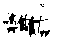
\includegraphics[height=3cm]{images/shepherds.png}\hfill\mbox{}

